\section{Virtual Development Environment}
\label{sec:VDE}

Da ich es für besser halte möglichst viel mit virtuellen Instanzen zu arbeiten, habe ich Jenkins und alle benötigten Plugins, Module, usw. auf diese Art und Weise installiert. Hierfür habe ich die gängige Software Ruby \textbf{Vagrant} verwendet. Ich habe schon oft mit Vagrant gearbeitet und komme ziemlich gut damit zu recht, deswegen gab es auch hier keine große Lernkurve. 

Grundsätzlich besteht die gesamte virtuelle Umgebung aus zwei Skripten die sich in dem Ordner vagrant in meinem Projekt befinden. Die Skripten sind einerseits das \textbf{Vagrantfile}, welches das grundsätzliche konfigurieren der Machine handled, und andererseits ein \textbf{Shellskript}, welches sich um die Installation der benötigten Software kümmert. \\ \\

\lstinputlisting[caption=Vagrantfile]{../../vagrant/Vagrantfile}
\clearpage
\lstinputlisting[caption=install.sh, style=Bash]{../../vagrant/install.sh}

\newpage

Nachdem die virtuelle Umgebung eingerichtet und konfiguriert ist kann sie nun mit dem Browser unter \textbf{127.0.0.1:8080} aufgerufen werden. Hier wird man mit dem Startbilschirm von Jenkins begrüßt. Man muss jetzt die Schritte durchführen, die im Part 3 des Tutorials sind - das heißt, die konfiguration von Jenkins.

Zunächst erstellt man ein Projekt, danach installiert man die benötigten Plugins, Cobertura, Git, Violations. Die konfiguration habe ich genau so gemacht wie es im tutorial beschrieben wurde. 

\vfill
\begin{figure}[h!]
	\caption{Erstellen des Projekts}
	\centering
	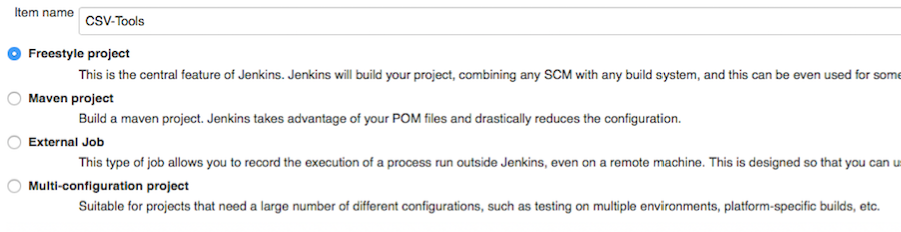
\includegraphics[width=\textwidth]{images/jenkins_config1.png}
\end{figure}

\begin{figure}[h!]
	\caption{Installation der Plugins}
	\centering
	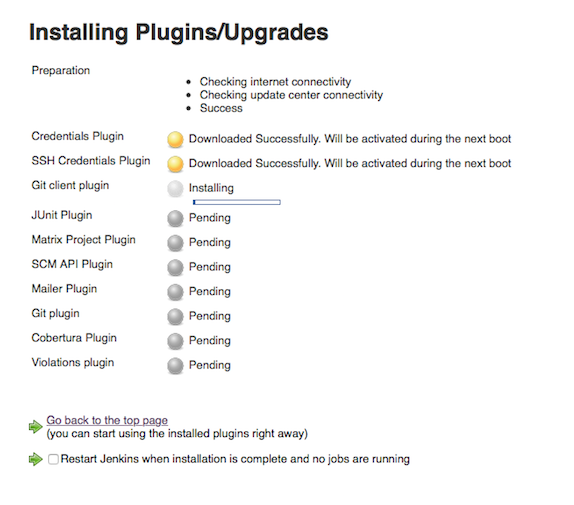
\includegraphics[width=0.6\textwidth, height=0.4\textheight]{images/jenkins_config2.png}
\end{figure}

Kommen wir nun zur eigentlichen konfiguration von Jenkins mit dem Projekt, in den folgenden Chaptern dieses Dokuments wird auf dies näher eingegangen.

\begin{figure}[h!]
	\caption{Projekt Konfiguration 1}
	\centering
	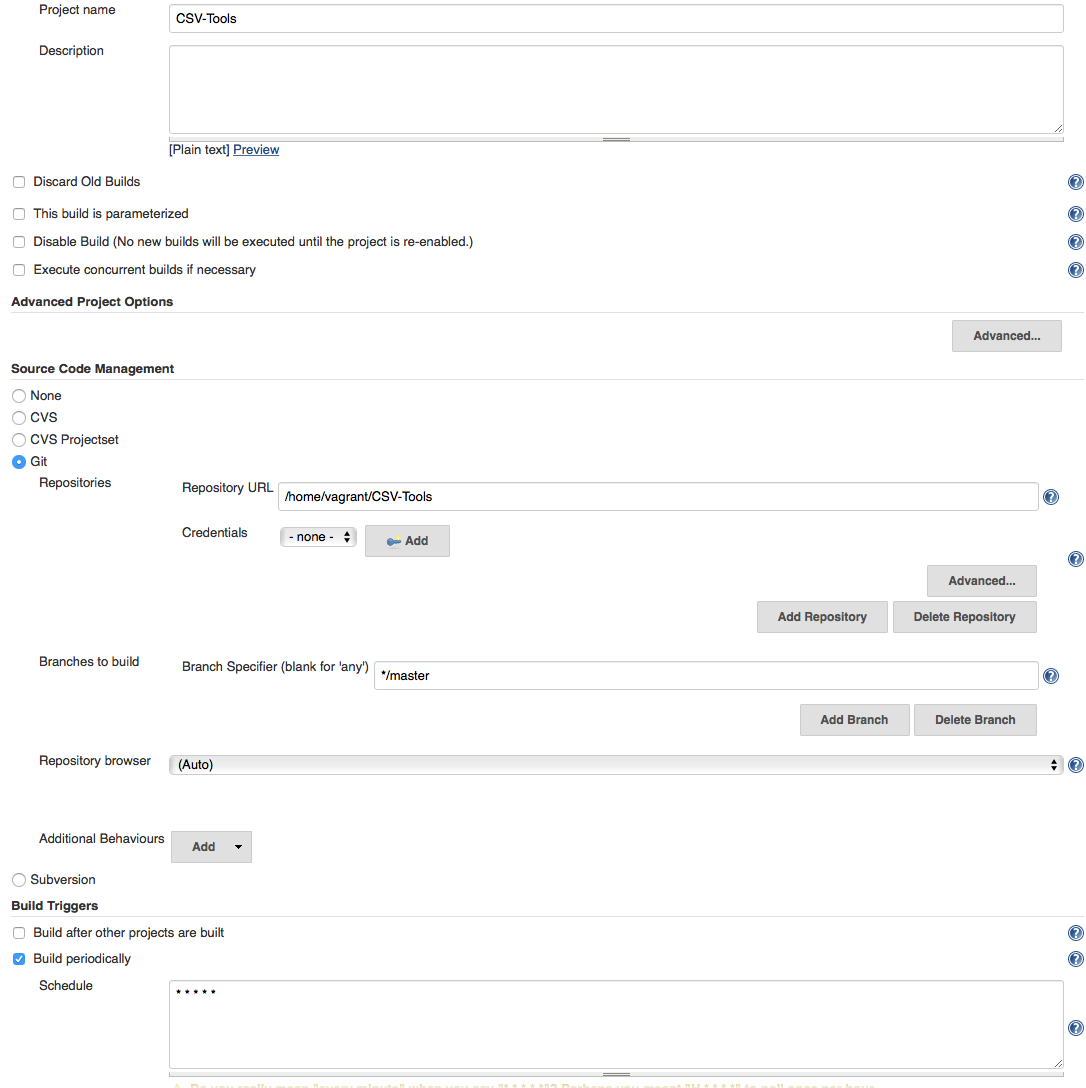
\includegraphics[width=\textwidth, height=0.8\textheight]{images/jenkins_projectConfig1.png}
\end{figure}

\begin{figure}[h!]
	\caption{Projekt Konfiguration 3}
	\centering
	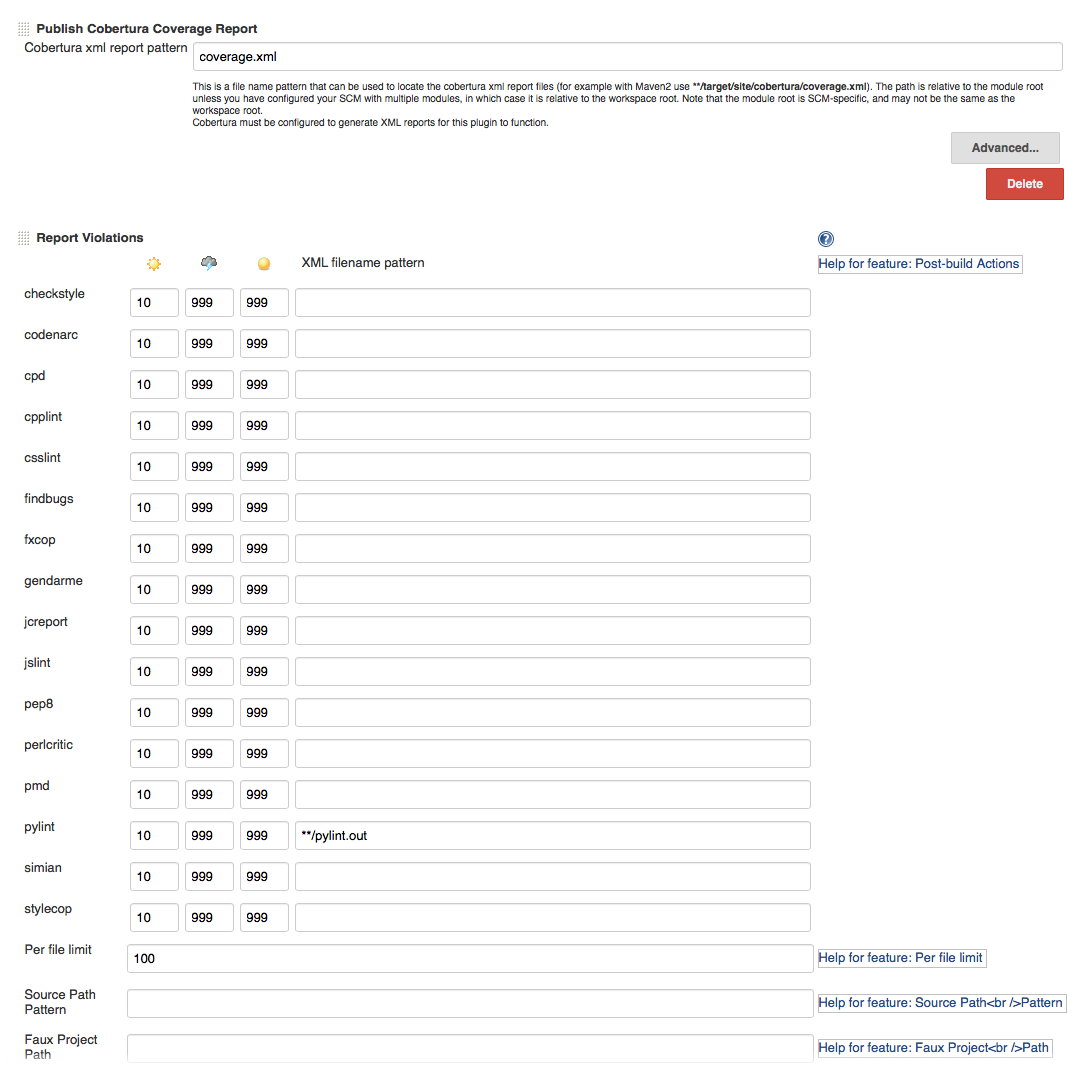
\includegraphics[width=\textwidth, height=0.8\textheight]{images/jenkins_projectConfig3.png}
\end{figure}
\vfill
\clearpage

Bezüglich des vom Tutorial abweichendem \textbf{Execute Shell Script} gibt es in einer späteren Section kommentare.

\begin{figure}[h!]
	\caption{Projekt Konfiguration 2}
	\centering
	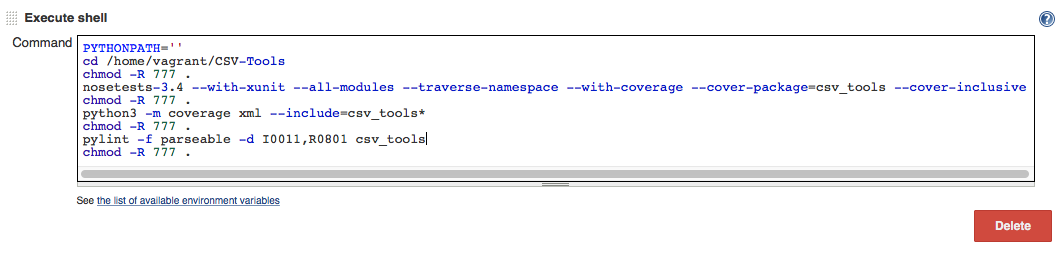
\includegraphics[width=\textwidth]{images/jenkins_projectConfig2.png}
\end{figure}